\part{Object-oriented programming}
\label{part:oop}

\section{Object-oriented programming}

\subsection{Class}

\begin{frame}{Class}{}
  \begin{definition}[Class]
    A \strong{class} is a user-defined type whose declaration begins with \lstinline!class! or \lstinline!struct!.
  \end{definition}

  \begin{block}{Remark}
    \lstinline!struct! and \lstinline!class! are indistinguishable in C++, except that the default access mode and default inheritance mode are \lstinline!public! if class declaration uses \lstinline!struct! and private if the class declaration uses \lstinline!class!.
  \end{block}
\end{frame}

\begin{frame}{Class members}{}
  \begin{block}{Class members}
    A class can have the following kinds of members:
    \begin{enumerate}
    \item
      Data members
      \begin{itemize}
      \item
        Non-static data members, including bit fields
      \item
        Static data members (\lstinline!static!)
      \end{itemize}
    \item
      Member functions
      \begin{itemize}
      \item
        Non-static member functions
      \item
        Static member functions (\lstinline!static!)
      \end{itemize}
    \item
      Nested types
      \begin{itemize}
      \item
        Nested classes and enumerations defined within the class definition
      \item
        Aliases of existing types, defined with \lstinline!typedef! or type alias declarations
      \end{itemize}
    \item
      Enumerators from all unscoped enumerations defined within the class
    \item
      Member templates (variable\Since{14}, class or function templates)
    \end{enumerate}
  \end{block}
\end{frame}

\begin{frame}{Class members}{}
  \begin{example}[Class members]
    \sourceinput{snippets/class_members.cc}
  \end{example}
\end{frame}


\subsection{Constructors}

\subsubsection{Constructor and member initializer list}

\begin{frame}{Constructor}{}
  \begin{definition}[Constructor]
    A \strong{constructor} is a special non-static member function of a class that is used to initialize objects of its class type.
  \end{definition}

  \begin{block}{Remarks}
    \begin{itemize}
    \item
      Constructors have no names and cannot be called directly
    \item
      They are invoked when initialization takes place
    \end{itemize}
  \end{block}

  \begin{block}{Special kinds of constructors}
    \begin{itemize}
    \item
      Converting constructors (without \lstinline!explicit! specifier)
    \item
      Default constructor (without arguments)
    \item
      Copy constructor and move constructor (with another object of the same type as the argument)
    \end{itemize}
  \end{block}
\end{frame}

\begin{frame}{Initialization order}{}
  \begin{block}{Initialization order}
    \begin{enumerate}
    \item
      Initialization of virtual bases
      \begin{itemize}
      \item
        Only in the most derived class of the object that's being constructed
      \item
        In depth-first left-to-right traversal of the base class declarations
      \end{itemize}
    \item
%       \label{lst:initbase}
      Initialization of direct bases
      \begin{itemize}
      \item
        In left-to-right order
      \end{itemize}
    \item
%       \label{lst:initdatamembers}
      Initialization of non-static data members
      \begin{itemize}
      \item
        In order of declaration in the class definition
      \end{itemize}
    \item
      Execution of the body of the constructor
    \end{enumerate}
%     Step~\ref{lst:initbase} to \ref{lst:initdatamembers} can be done in the \emph{member initializer list}.
  \end{block}

  % TODO: default member initializer
\end{frame}


\begin{frame}{Member initializer list}{}
  \begin{definition}[Member initializer list]
    In the definition of a constructor of a class, a \strong{member initializer list} specifies the \emph{non-default} initializers for direct and virtual base subobjects and non-static data members.
  \end{definition}

  \begin{block}{Remark}
    The list may not be in the same order as the members but compilers issue a warning in that case.
  \end{block}
\end{frame}

\begin{frame}{Member initializer list}{}
  \begin{example}[Member initializer list]
    \sourceinput{snippets/member_initializer_list.cc}
  \end{example}
\end{frame}

\subsubsection{Converting constructor}

\begin{frame}{Converting constructor and explicit constructors}{}
  \begin{definition}[Converting constructor]
    A \strong{converting constructor} is not declared with the specifier \lstinline!explicit!
  \end{definition}

  \begin{block}{Converting constructors and explicit constructors}
    \begin{itemize}
    \item
      Both kind of constructors are considered in direct initialization
    \item
      Converting constructors are also considered in copy initialization (conversion)
    \end{itemize}
  \end{block}
\end{frame}

\begin{frame}{Converting constructor}{}
  \begin{example}[Converting constructor]
    \sourceinput{snippets/converting_constructor.cc}
  \end{example}
\end{frame}

\begin{frame}{Explicit constructor}{}
  \begin{example}[Explicit constructor]
    \sourceinput{snippets/explicit_constructor.cc}
  \end{example}
\end{frame}

\subsubsection{Default constructor}

\begin{frame}{Default constructor}{}
  \begin{definition}[Default constructor]
    A default constructor is a constructor that can be called with no arguments (either defined with an empty parameter list, or with default arguments provided for every parameter).
  \end{definition}

  \begin{block}{Default constructor}
    \begin{itemize}
    \item
      If no user-declared constructors of any kind are provided for a class, the compiler will always declare a default constructor
    \item
      A default constructor can be:
      \begin{itemize}
      \item
        Explicitely declared with \lstinline! = default! after its declaration
      \item
        Explicitely deleted with \lstinline! = delete! after its declaration
      \end{itemize}
    \end{itemize}
  \end{block}
\end{frame}

\begin{frame}{Default constructor}{}
  \begin{example}[Default constructor]
    \sourceinput{snippets/default_constructor.cc}
  \end{example}
\end{frame}


\subsubsection{Copy and move constructors}

\begin{frame}{Copy constructor}{}
  \begin{definition}[Copy constructor]
    A copy constructor of class \lstinline!T! is a non-template constructor whose first parameter is (generally) \lstinline!const T&!
  \end{definition}

  \begin{block}{Copy constructor}
    \begin{itemize}
    \item
      If a copy constructor is not declared, it is implicitly declared, if possible or it is implicitly deleted otherwise
    \item
      A copy constructor can be:
      \begin{itemize}
      \item
        Explicitely declared and defaulted with \lstinline! = default! after its declaration
      \item
        Explicitely deleted with \lstinline! = delete! after its declaration
      \end{itemize}
    \item
      A copy constructor is used in the following cases (\lstinline!a! and \lstinline!b! are of type \lstinline!T!):
      \begin{itemize}
      \item
        Initialization: \lstinline!T a = b;! or \lstinline!T a(b);!
      \item
        Function argument passing: \lstinline!f(a);!, where \lstinline!f! is \lstinline!void f(T t)!
      \item
        Function return: \lstinline!return a;! inside a function such as \lstinline!T f()!, where type \lstinline!T! has no move constructor
      \end{itemize}
    \end{itemize}
  \end{block}
\end{frame}


\begin{frame}{Move constructor}{}
  \begin{definition}[Move constructor]
    A move constructor of class \lstinline!T! is a non-template constructor whose first parameter is (generally) \lstinline!T&&!
  \end{definition}

  \begin{block}{Move constructor}
    \begin{itemize}
    \item
      If a move constructor is not declared, it is implicitly declared, if possible or it is implicitly deleted otherwise
    \item
      A move constructor can be:
      \begin{itemize}
      \item
        Explicitely declared and defaulted with \lstinline! = default! after its declaration
      \item
        Explicitely deleted with \lstinline! = delete! after its declaration
      \end{itemize}
    \item
      A move constructor is used in the following cases (\lstinline!a! and \lstinline!b! are of type \lstinline!T!):
      \begin{itemize}
      \item
        Initialization: \lstinline!T a = std::move(b);! or \lstinline!T a(std::move(b));!
      \item
        Function argument passing: \lstinline!f(std::move(a));!, where \lstinline!f! is \lstinline!void f(T t)!
      \item
        Function return: \lstinline!return a;! inside a function such as \lstinline!T f()!, where type \lstinline!T! has a move constructor
      \end{itemize}
    \end{itemize}
  \end{block}
\end{frame}

\begin{frame}{Copy and move constructors}{}
  \begin{example}[Copy and move constructors]
    \sourceinput{snippets/copy_move_constructors.cc}
  \end{example}
\end{frame}

% TODO: copy asssignment and move assignment

\subsection{Destructors}

\subsubsection{Destructor}

\begin{frame}{Destructor}{}
  \begin{definition}[Destructor]
    A \strong{destructor} is a special member function that is called when the lifetime of an object ends. The purpose of the destructor is to free the resources that the object may have acquired during its lifetime.

    {
      \hfill\lstinline[mathescape]!\~ $ClassName$ ()!\hfill
    }
  \end{definition}

  \begin{block}{Destruction sequence}
    \begin{enumerate}
    \item
      Execution of the body of the destructor
    \item
      Destruction of non-static data members
      \begin{itemize}
      \item
        In reverse order of declaration in the class definition
      \end{itemize}
    \item
      Destruction of direct bases
      \begin{itemize}
      \item
        In reverse order of construction, i.e. right-to-left
      \end{itemize}
    \item
      Destruction of virtual bases
      \begin{itemize}
      \item
        Only in the most derived class of the object that's being destroyed
      \end{itemize}
    \end{enumerate}
  \end{block}
\end{frame}

\begin{frame}{Destructor call}{}
  \begin{block}{Destructor call}
    The destructor is called whenever an object's lifetime ends, which includes:
    \begin{itemize}
    \item
      program termination, for objects with static storage duration
    \item
      thread exit, for objects with thread-local storage duration
    \item
      end of scope, for objects with automatic storage duration and for temporaries whose life was extended by binding to a reference
    \item
      delete expression, for objects with dynamic storage duration
    \item
      end of the full expression, for nameless temporaries
    \item
      stack unwinding, for objects with automatic storage duration when an exception escapes their block, uncaught
    \item[$\to$]
      Most of the time, the destructor is called automatically!
    \end{itemize}
  \end{block}
\end{frame}

\begin{frame}{Destructor}{}
  \begin{example}[Destructor]
    \sourceinput{snippets/destructor.cc}
  \end{example}
\end{frame}


\subsubsection{Rule of Three, Rule of Five, Rule of Zero}

\begin{frame}{Rule of Three}{}
  \begin{definition}[Rule of Three]
    If a class requires
    \begin{itemize}
    \item
      a user-defined destructor,
    \item
      a user-defined copy constructor,
    \item
      or a user-defined copy assignment operator,
    \end{itemize}
    it almost certainly requires all three.
  \end{definition}

  \begin{block}{Reason}
    The implicitly-defined special member functions are typically incorrect if the class is managing a resource whose handle is an object of non-class type (raw pointer, POSIX file descriptor, etc), whose destructor does nothing and copy constructor/assignment operator performs a "shallow copy" (copy the value of the handle, without duplicating the underlying resource).
  \end{block}
\end{frame}

\begin{frame}{Rule of Five}{}
  \begin{example}[Rule of Three]
    \sourceinput{snippets/rule_of_three.cc}
  \end{example}
\end{frame}

\begin{frame}{Rule of Five}{}
  \begin{definition}[Rule of Five]
    Because the presence of a user-defined destructor, copy-constructor, or copy-assignment operator prevents implicit definition of the move constructor and the move assignment operator, any class for which move semantics are desirable, has to declare all five special member functions
  \end{definition}

  \begin{block}{Remark}
    Unlike Rule of Three, failing to provide move constructor and move assignment is usually not an error, but a missed optimization opportunity.
  \end{block}
\end{frame}

\begin{frame}{Rule of Five}{}
  \begin{example}[Rule of Five]
    \sourceinput{snippets/rule_of_five.cc}
  \end{example}
\end{frame}

\begin{frame}{Rule of Zero}{}
  \begin{definition}[Rule of Zero]
    Classes that have custom destructors, copy/move constructors or copy/move assignment operators should deal exclusively with ownership (which follows from the Single Responsibility Principle). Other classes should not have custom destructors, copy/move constructors or copy/move assignment operators.
  \end{definition}
\end{frame}

\begin{frame}{Rule of Zero}{}
  \begin{example}[Rule of Zero]
    \sourceinput{snippets/rule_of_zero.cc}
  \end{example}
\end{frame}

\subsubsection{Resource Acquisition Is Initialization (RAII)}

\begin{frame}{Resource Acquisition Is Initialization (RAII)}{}
  \begin{definition}[Resource Acquisition Is Initialization (RAII)]
    \strong{Resource Acquisition Is Initialization} (RAII), is a C++ programming technique which binds the life cycle of a resource that must be acquired before use to the lifetime of an object.
  \end{definition}

  \begin{examples}[Resources where RAII could be used]
    \begin{itemize}
    \item
       Allocated heap memory
    \item
       Thread of execution
    \item
       Open socket
    \item
       Open file
    \item
       Locked mutex
    \item
       Disk space
    \item
       Database connection
    \end{itemize}
  \end{examples}
\end{frame}

\begin{frame}{RAII in Practice}{}
  \begin{block}{RAII in Practice}
    \begin{itemize}
    \item
      Encapsulate each resource into a class, where
      \begin{itemize}
      \item
        the constructor acquires the resource and establishes all class invariants or throws an exception if that cannot be done
      \item
        the destructor releases the resource and never throws exceptions
      \end{itemize}
    \item
      Always use the resource via an instance of a RAII-class that either
      \begin{itemize}
      \item
        has automatic storage duration or temporary lifetime itself, or
      \item
        has lifetime bounded by the lifetime of an automatic or temporary object
      \end{itemize}
    \end{itemize}
  \end{block}

  \begin{block}{Remark}
    Classes with \lstinline!open()!/\lstinline!close()!, \lstinline!lock()!/\lstinline!unlock()!, or \lstinline!init()!/\lstinline!destroy()! member functions are typical examples of non-RAII classes
  \end{block}
\end{frame}


\begin{frame}{Resource Acquisition Is Initialization}{}
  \begin{example}[Resource Acquisition Is Initialization]
    \sourceinput{snippets/raii.cc}
  \end{example}
\end{frame}

% - Others might be more helpful in grokking what it really is, such as "Constructor Acquires, Destructor Releases" (CADRe) or "Scope-based Resource Management" (SBRM).

\subsection{Inheritance}

\subsubsection{Derived classes}

\begin{frame}{Derived Classes}{}
  \begin{block}{Derived Classes}
    Any class may be declared as \emph{derived} from one or more \emph{base classes} which, in turn, may be derived from their own base classes, forming an inheritance hierarchy. Each base class:
    \begin{itemize}
    \item
      may have an access specifer: \lstinline!public!, \lstinline!protected!, \lstinline!private!
    \item
      may be declared \lstinline!virtual!
    \end{itemize}
  \end{block}

  \begin{block}{Remark}
    If the access specifier is omitted, it defaults to:
    \begin{itemize}
    \item
      \lstinline!public! for \lstinline!struct!
    \item
      \lstinline!private! for \lstinline!class!
    \end{itemize}
  \end{block}
\end{frame}

\begin{frame}{Derived Classes}{}
  \begin{example}[Derived Classes]
    \sourceinput{snippets/derived_class.cc}
  \end{example}
\end{frame}

\subsubsection{Virtual base classes}

\begin{frame}{Virtual base class}{}
  \begin{block}{Virtual base class}
    For each distinct base class that is specified \lstinline!virtual!, the most derived object contains only one base class subobject of that type, even if the class appears many times in the inheritance hierarchy (as long as it is inherited \lstinline!virtual! every time).
  \end{block}

  \begin{example}[Famous example of virtual base class]
    \begin{center}
    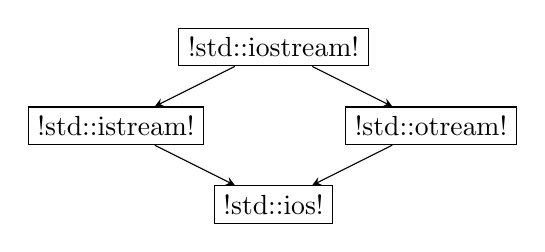
\begin{tikzpicture}
      \node[draw] (IO) at ( 0, 0) { \lstinline!std::iostream! } ;
      \node[draw] (I) at (-2,-1) { \lstinline!std::istream! } ;
      \node[draw] (O) at ( 2,-1) { \lstinline!std::otream! } ;
      \node[draw] (B) at ( 0,-2) { \lstinline!std::ios! } ;

      \draw[->,>=stealth] (IO) -- (I) ;
      \draw[->,>=stealth] (IO) -- (O) ;
      \draw[->,>=stealth] (I) -- (B) ;
      \draw[->,>=stealth] (O) -- (B) ;
    \end{tikzpicture}
    \end{center}
  \end{example}
\end{frame}

\begin{frame}{Virtual base class}{}
  \begin{example}[Virtual base class]
    \sourceinput{snippets/virtual_base_class.cc}
  \end{example}
\end{frame}

% TODO: initialization of virtual base class?


\subsubsection{Empty Base Optimization (EBO)}

\begin{frame}{Empty Base Optimization (EBO)}{}
  \begin{block}{Empty Base Optimization (EBO)}
    \strong{Empty Base Optimization} (EBO) allows the size of an empty base subobject to be zero
  \end{block}

  \begin{block}{Explanation}
    The size of any object or member subobject is required to be at least 1 even if the type is an empty class, in order to be able to guarantee that the addresses of distinct objects of the same type are always distinct.

    However, base class subobjects are not so constrained, and can be completely optimized out from the object layout
  \end{block}
\end{frame}

\begin{frame}{Empty Base Optimization}{}
  \begin{example}[Empty Base Optimization]
    \sourceinput{snippets/ebo.cc}
  \end{example}
\end{frame}


\subsection{Polymorphism}

%
% vptr/vtable (https://www.geeksforgeeks.org/commonly-asked-c-interview-questions-set-1/)
% override
% RTTI

%   - virtual destructor

\subsection{PImpl My Ride}


% - pimpl
% https://cpppatterns.com/patterns/pimpl.html
% https://wiki.qt.io/D-Pointer

\subsection{\texttt{const} correctness}

%
% - const correctness
% https://isocpp.org/wiki/faq/const-correctness
%
%


% (N)RVO

% \begin{frame}{}{}
%   \begin{block}{}
%     \begin{itemize}
%     \item
%     \item
%     \end{itemize}
%   \end{block}
% \end{frame}
